%% Version 6.1, 1 September 2021
%
%%%%%%%%%%%%%%%%%%%%%%%%%%%%%%%%%%%%%%%%%%%%%%%%%%%%%%%%%%%%%%%%%%%%%%
% TemplateV6.1.tex --  LaTeX-based blank template for submissions to the 
% American Meteorological Society
%
%%%%%%%%%%%%%%%%%%%%%%%%%%%%%%%%%%%%%%%%%%%%%%%%%%%%%%%%%%%%%%%%%%%%%
% PREAMBLE
%%%%%%%%%%%%%%%%%%%%%%%%%%%%%%%%%%%%%%%%%%%%%%%%%%%%%%%%%%%%%%%%%%%%%

%% Start with one of the following:
% 1.5-SPACED VERSION FOR SUBMISSION TO THE AMS
\documentclass{ametsocV6.1}

% TWO-COLUMN JOURNAL PAGE LAYOUT---FOR AUTHOR USE ONLY
% \documentclass[twocol]{ametsocV6.1}

%%%%%%%%%%%%%%%%%%%%%%%%%%%%%%%%

%%% To be entered by author:

%% May use \\ to break lines in title:

\title{More observation and selected VOCs}

%% Enter authors' names and affiliations as you see in the examples below.
%
%% Use \correspondingauthor{} and \thanks{} (\thanks command to be used for affiliations footnotes, 
%% such as current affiliation, additional affiliation, deceased, co-first authors, etc.)
%% immediately following the appropriate author.
%
%% Note that the \correspondingauthor{} command is NECESSARY.
%% The \thanks{} commands are OPTIONAL.
%
%% Enter affiliations within the \affiliation{} field. Use \aff{#} to indicate the affiliation letter at both the
%% affiliation and at each author's name. Use \\ to insert line breaks to place each affiliation on its own line.

%\authors{Author One,\aff{a}\correspondingauthor{Author One, email@email.com} 
%Author Two,\aff{a} 
%Author Three,\aff{b} 
%Author Four,\aff{a} 
%Author Five\thanks{Author Five's current affiliation: NCAR, Boulder, Colorado},\aff{c} 
%Author Six,\aff{c} 
%Author Seven,\aff{d}
% and Author Eight\aff{a,d}
%}
%
%\affiliation{\aff{a}{First Affiliation}\\
%\aff{b}{Second Affiliation}\\
%\aff{c}{Third Affiliation}\\
%\aff{d}{Fourth Affiliation}
%}

\authors{Haoxing Ju\aff{a}\correspondingauthor{Author One, email@email.com}}

\affiliation{\aff{a}{Nanjing University}}

%%%%%%%%%%%%%%%%%%%%%%%%%%%%%%%%%%%%%%%%%%%%%%%%%%%%%%%%%%%%%%%%%%%%%
% ABSTRACT
%
% Enter your abstract here
% Abstracts should not exceed 250 words in length!
%
 
\abstract{Enter the text of your abstract here.}

\begin{document}

%% Necessary!
\maketitle

%%%%%%%%%%%%%%%%%%%%%%%%%%%%%%%%%%%%%%%%%%%%%%%%%%%%%%%%%%%%%%%%%%%%%
% SIGNIFICANCE STATEMENT/CAPSULE SUMMARY
%%%%%%%%%%%%%%%%%%%%%%%%%%%%%%%%%%%%%%%%%%%%%%%%%%%%%%%%%%%%%%%%%%%%%
%
% If you are including an optional significance statement for a journal article or a required capsule summary for BAMS 
% (see www.ametsoc.org/ams/index.cfm/publications/authors/journal-and-bams-authors/formatting-and-manuscript-components for details), 
% please apply the necessary command as shown below:
%
% Significance Statement (all journals except BAMS)
%
%\statement
%	 Enter significance statement here, no more than 120 words. See \url{www.ametsoc.org/index.cfm/ams/publications/author-information/significance-statements/} for details.
%
%% Capsule (BAMS only)
%%
%\capsule
%       Enter BAMS capsule here, no more than 30 words. See \url{www.ametsoc.org/index.cfm/ams/publications/author-information/formatting-and-manuscript-components/#capsule} for details.
%
%% * * If using twocol mode, you will need to use the commands "twocolsig" and "twocolcapsule" in place of "sig" and "capsule"
%%      to ensure that the text box correctly spans across both columns.
%

%%%%%%%%%%%%%%%%%%%%%%%%%%%%%%%%%%%%%%%%%%%%%%%%%%%%%%%%%%%%%%%%%%%%%
% MAIN BODY OF PAPER
%%%%%%%%%%%%%%%%%%%%%%%%%%%%%%%%%%%%%%%%%%%%%%%%%%%%%%%%%%%%%%%%%%%%%
%

%% In all cases, if there is only one entry of this type within
%% the higher level heading, use the star form: 
%%

\section{Introduction}
Volatile organic compounds (VOCs) have been known for their active role in photochemical process as being major precursors of secondary PM2.5, troposhere ozone\citep{Wu_2018}, and thus China's Ministry of Ecology and Environment (MEE) has listed volatile organic compounds (VOCs) among the key pollutants to be controlled in the series plans since 2013. Chemical Transport Model (CTM) is powerful tool to simulate atmosphere pollution and support political desicions, but VOCs in CTM are far from being fully simulated. Errors come from various part, (haoxing: here we need more ...). Considering their important role in precursors for many pollutions, and their great uncertainty in CTM simulation, tackling VOCs uncertainty in CTMs is critical to improve forecast.(haoxing: need polish here...)

Data assimilation has achieved great success in reducing uncertainty in meteorological modelling since Last centery, and in recent years has also extended its success in CTM. One major difference in meteorology model assimilation and CTM assimilation is the additional emission field in CTM. Unlike meteorology model, in which initial errors have determinant influence in error growing, in CTM, emission error plays an equal role as initial state variable error, or even more crucial, as initial error fading over time\citep{Sandu_2011}. Thus, assimilating IC and emission at the same time is needed, and will get a better assimilation performance compared to only assimilate IC/Emission\citep{Elbern_2007, Tang_2011}.

But, when it comes to assimilating VOCs, many difficulties occure. Firstly, observation of VOCs is rare, compared with the six main pollution species(PM2.5, PM10, Ozone, NO2, SO2, CO) which, according to MEP, have over 1500 station across china providing hourly observation. Even we conduct several VOCs observation by ourselves, the short lifetime of VOCs will also limit the localization scale in assimilation\citep{Koohkan_2013}, making it hard to be directly used in models with large domain, and also make it hard to do a validation. Secondly, there exist over houndards of VOCs species in model state variable, each possess its own chemical character, and their classification differ among several gas-phase chemical mechanism(haoxing: maybe we can extend more) . What's worse, VOCs have highly non-linear reactions among themselves, Ozone, NOx, SOA(PM2.5), and many other state variables. In an assimilation framework with several linear approximation, it will make assimilation result diverge quickly from truth\citep{Tang_2016}. All of these make VOCs assimilation hard. Previous works tend to view all VOCs species as a whole, and assimilate it without considering the differences between VOC species\citep{Tang_2011, Ma_2019, Xing_2020}. This simplification will certainly bring in extra uncertainly, and make this kind of VOC assimilation not work or even worse in some cases.

\section{Model configurations and data assimilation system}
We use WRF-Chem versioin 3.6.1 to simulate chemical and meteorological variables\citep{Grell_2005}. WRF-Chem is an 'online' model with fully-coupled chemical and meteorological fields, which means a perturb in meteorological fields can have impact on chemical fields, and vise versa. The EnSRF\citep{Whitaker_2002} with its expansion to chem and emission component\citep{Schwartz_2014, Peng_2017} is chosen to construct the data assimilation system.

In most CTMs, including WRF-Chem, emission fields are treated as external forcing, rather than state variables. So, in order to use concentration observations and assimilation system to constrain emission, we need to extend emission as part of model state variables, and introduce a forecasting model M to let it develop with time. Peng has developed a emission forecast model with scaling factor as state variables, and its advantage has been proved in multi-species emission inversion.\citep{Peng_2017, Peng_2018}. Here, we take Peng's forecast model to let emission scaling factors develop with time.

Section 2.1 will describle the WRF-Chem model settings and emission forecast model with more details, and section 2.2 will further describle the assimilation system settings.

\subsection{WRF-Chem model setting}

% Table 1 for wrf-chem paramenterization setting. See Peng2018 for an example.
% Table 2 for RADM2 NMVOCs speciation in model. (14 VOCs we use).

Figure for domain setting and chem observation station distribution. More detailed description of station observations we use can be seen at section 3.2.

The update of source emissions through assimilation of chemical observations follows\citep{Peng_2017}, detailed description will not expand here.

\begin{figure}
% haoxing: need to adjust for better showing. maybe add a subplot for YRD domain?
    \centerline{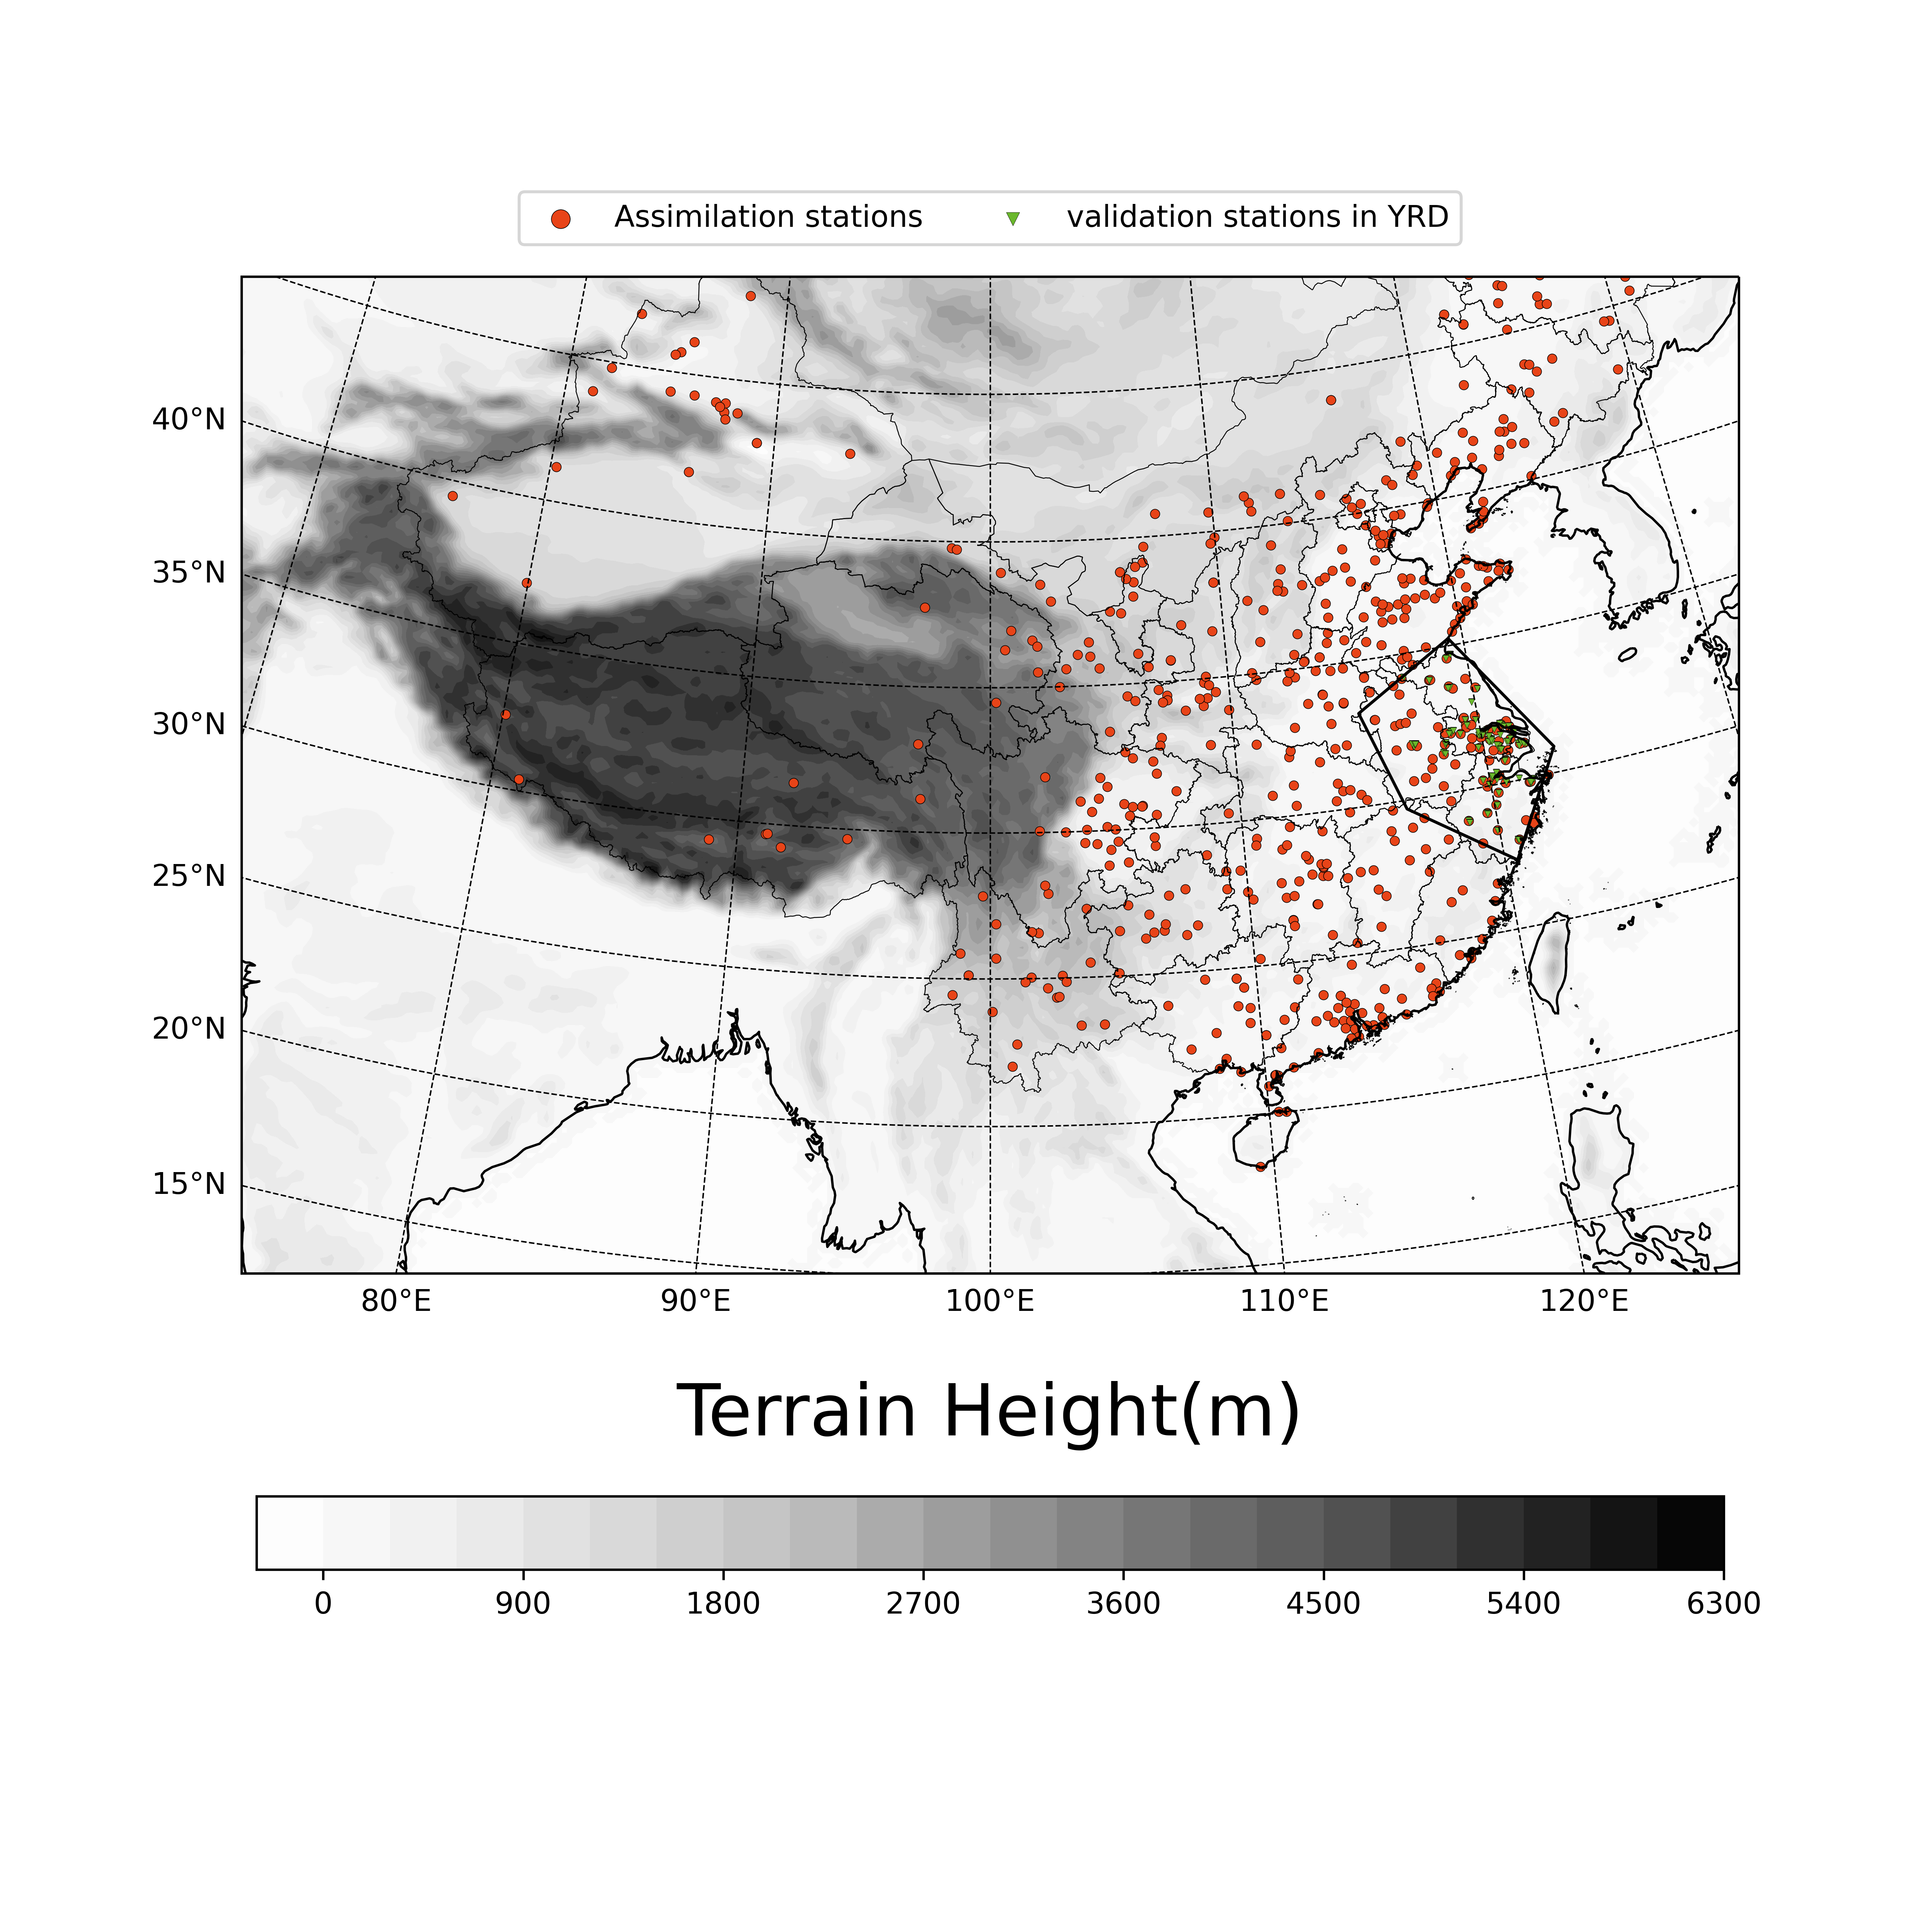
\includegraphics[width=30pc,angle=0]{figure/domain_station_yrd_withvalid.png}}
    \caption{domain and station}\label{fig1}
\end{figure}

\subsection{data assimilation setting}

\section{Observations}

\subsection{meteorology}

\subsection{chem}

\subsection{emission}
Mainland China: The hourly prescribed anthropogenic emission is obtained from the Multi‐resolution Emission Inventory for China (MEIC v1.3) \citep{Li_2017, Zheng_2018} in July 2017, which is the most updated dataset. In areas out of mainland china, we use EDGARv6.1 in July 2017.

\section{Experiment design}

\section{Results}
% \section{Section title}
% \subsection{subsection one}
% text...
% \subsection{subsection two}
% \section{Section title}

%%%
% \section{First primary heading}

% \subsection{First secondary heading}

% \subsubsection{First tertiary heading}

% \paragraph{First quaternary heading}

%%%%%%%%%%%%%%%%%%%%%%%%%%%%%%%%%%%%%%%%%%%%%%%%%%%%%%%%%%%%%%%%%%%%%
% TABLES---INSERT NEAR IN-TEXT DISCUSSION
%%%%%%%%%%%%%%%%%%%%%%%%%%%%%%%%%%%%%%%%%%%%%%%%%%%%%%%%%%%%%%%%%%%%%
%%  Enter tables near where they are discussed within the document. 
%%  Please place tables before/after paragraphs, not within a paragraph.
%%
%
%\begin{table}[t]
%\caption{This is a sample table caption and table layout.  Enter as many tables as
%  necessary at the end of your manuscript. Table from Lorenz (1963).}\label{t1}
%\begin{center}
%\begin{tabular}{ccccrrcrc}
%\hline\hline
%$N$ & $X$ & $Y$ & $Z$\\
%\hline
% 0000 & 0000 & 0010 & 0000 \\
% 0005 & 0004 & 0012 & 0000 \\
% 0010 & 0009 & 0020 & 0000 \\
% 0015 & 0016 & 0036 & 0002 \\
% 0020 & 0030 & 0066 & 0007 \\
% 0025 & 0054 & 0115 & 0024 \\
%\hline
%\end{tabular}
%\end{center}
%\end{table}

%%%%%%%%%%%%%%%%%%%%%%%%%%%%%%%%%%%%%%%%%%%%%%%%%%%%%%%%%%%%%%%%%%%%%
% FIGURES---INSERT NEAR IN-TEXT DISCUSSION
%%%%%%%%%%%%%%%%%%%%%%%%%%%%%%%%%%%%%%%%%%%%%%%%%%%%%%%%%%%%%%%%%%%%%
%%  Enter figures near where they are discussed within the document.
%%  Please place figures before/after paragraphs, not within a paragraph.
% %
%
%\begin{figure}[t]
%  \noindent\includegraphics[width=19pc,angle=0]{figure01.pdf}\\
%  \caption{Enter the caption for your figure here.  Repeat as
%  necessary for each of your figures. Figure from \protect\citep{Knutti2008}.}\label{f1}
%\end{figure}

\clearpage
%%%%%%%%%%%%%%%%%%%%%%%%%%%%%%%%%%%%%%%%%%%%%%%%%%%%%%%%%%%%%%%%%%%%%
% ACKNOWLEDGMENTS
%%%%%%%%%%%%%%%%%%%%%%%%%%%%%%%%%%%%%%%%%%%%%%%%%%%%%%%%%%%%%%%%%%%%%
\acknowledgments
%  Keep acknowledgments (note correct spelling: no ``e'' between the ``g'' and
% ``m'') as brief as possible. In general, acknowledge only direct help in
%  writing or research. Financial support (e.g., grant numbers) for the work done, 
%  for an author, or for the laboratory where the work was performed must be 
%  acknowledged here rather than as footnotes to the title or to an author's name.
%  Contribution numbers (if the work has been published by the author's institution 
%  or organization) should be placed in the acknowledgments rather than as 
%  footnotes to the title or to an author's name.

%%%%%%%%%%%%%%%%%%%%%%%%%%%%%%%%%%%%%%%%%%%%%%%%%%%%%%%%%%%%%%%%%%%%%
% DATA AVAILABILITY STATEMENT
%%%%%%%%%%%%%%%%%%%%%%%%%%%%%%%%%%%%%%%%%%%%%%%%%%%%%%%%%%%%%%%%%%%%%
% 
%
\datastatement
%  The data availability statement is where authors should describe how the data underlying 
%  the findings within the article can be accessed and reused. Authors should attempt to 
%  provide unrestricted access to all data and materials underlying reported findings. 
%  If data access is restricted, authors must mention this in the statement. See
%  {http://www.ametsoc.org/PubsDataPolicy} for more info.

%%%%%%%%%%%%%%%%%%%%%%%%%%%%%%%%%%%%%%%%%%%%%%%%%%%%%%%%%%%%%%%%%%%%%
% APPENDIXES
%%%%%%%%%%%%%%%%%%%%%%%%%%%%%%%%%%%%%%%%%%%%%%%%%%%%%%%%%%%%%%%%%%%%%
%
%% If only one appendix, use

%\appendix

%% If more than one appendix, use \appendix[<letter>], e.g.,

%\appendix[A] 

%% Appendix title is necessary! For appendix title:

%\appendixtitle{Title of Appendix}

%%% Appendix section numbering (note, skip \section and begin with \subsection)
%
% \subsection{First primary heading}

% \subsubsection{First secondary heading}

% \paragraph{First tertiary heading}


%%%%%%%%%%%%%%%%%%%%%%%%%%%%%%%%%%%%%%%%%%%%%%%%%%%%%%%%%%%%%%%%%%%%%
% REFERENCES
%%%%%%%%%%%%%%%%%%%%%%%%%%%%%%%%%%%%%%%%%%%%%%%%%%%%%%%%%%%%%%%%%%%%%
% Make your BibTeX bibliography by using these commands:
\bibliographystyle{ametsocV6}
\bibliography{references}


\end{document}